\section{Theorie}

\subsection{Zielsetzung}

In dem folgenden Versuch soll mithilfe der Öltröopchenmethode nach Milikan
die Elementarladung $e\ua{0}$ bestimmt werden. Unter Verwendung der Faraday-Konstante
kann dann anschließend die Avogadro-Konstante errechnet werden.

\subsection{Theoretische Grundlagen}

Bei dem Milikan-Versuch werden Öltröpchen in das vertikale Feld eines Platten-Kondensators
gebracht. Da die Tröpchen bei der Zerstäubung mit einem ganzzahligen Vielfachen
der Elementarladung geladen werden, kann aus dem Verhalten bei verschiedenen
Feldeinstellungen die Elementarladung bestimmt werden.

Bei einem deaktivierten äußeren Feld wirken auf das Öltröpchen sowohl die
Gewichtskraft $\vec{F}\ua{g} = m \vec{g}$ als auch die Stokesche Reibungskraft durch die
Viskosität $\eta\ua{L}$ der Luft $\vec{F}\ua{R} = -6\pi r\eta\ua{L} v\ua{o}$.
Zusätzlich wird in den Formeln der Auftrieb durch die umgebende Luft beachtet,
welcher allerdings normalerweise vernachlässigt werden kann, da die Dichte der
Luft deutlich geringer ist als die des Öltröpchens. Für ein abgeschaltetes Feld
ergibt sich somit die folgende Kräftegleichung:

\begin{equation}
  \frac{4\pi}{3}r^3(\rho\ua{Oel}-\rho\ua{L})g = 6\pi\eta\ua{L}rv\ua{0}
  \label{eqn:Kräftegleichung_Ohne}
\end{equation}

Aus der Kräftegleichung lässt sich durch Umstellen somit auch der Radius des
Öltröpchens bestimmen:

\begin{equation}
  r = \sqrt{ \frac{9\eta\ua{L}v\ua{0}}{2g(\rho\ua{Oel}-\rho\ua{L})}}
  \label{eqn:Radius_Ohne}
\end{equation}

In Abbildung \ref{fig:Kräftegleichgewicht} sind die angreifenden Kräfte bei einem
geladenen Öltröpchen eingezeichnet. Die linke Abbildung zeigt ein parallel zu
Gravitationskraft gerichtetes Feld, während die rechte Abbildung ein der
Gravitationskraft entgegengesetztes Feld zeigt. Wenn man die verschiedenen
Kräfte nun in Relation setzt, lässt sich für beide Fälle eine Kräftegleichung
aufstellen, in der die elektrostatische Kraft $F\ua{el} = q \vec{E}$ berücksichtigt
wird.

\begin{figure}
  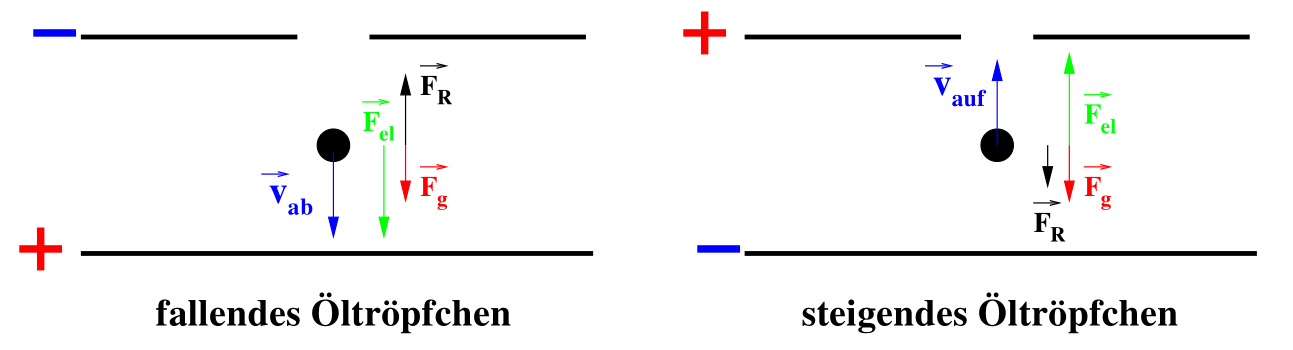
\includegraphics[width=\textwidth]{Pics/Kraefte_homogenes_Feld.png}
  \caption{Kräftegleichgewicht in einem homogenen elektrischen Feld \cite{anleitung01}.}
  \label{fig:Kräftegleichgewicht}
\end{figure}

Bei einem parallel zu $\vec{F}\ua{g}$ wirkenden elektrischen Feld stellt sich dabei
eine gleichförmige Sinkgeschwindigkeit $v\ua{down}$ ein, welche größer als die
Geschwindigkeit $v\ua{0}$ ohne elektrisches Feld ist:

\begin{equation}
  \frac{4\pi}{3}r^3(\rho\ua{Oel}-\rho\ua{L})g - 6\pi\eta\ua{L}rv\ua{down} = -qE
  \label{eqn:Kräftegleichung_parallel}
\end{equation}

Bei einem entgegengesetztem Feld stellt sich bei einer genügend hohen Feldstärke
eine Aufwärtsbewegung mit der Geschwindigkeit $v\ua{up}$ ein, für die sich
folgende Kräftegleichung ergibt:

\begin{equation}
  \frac{4\pi}{3}r^3(\rho\ua{Oel}+\rho\ua{L})g + 6\pi\eta\ua{L}rv\ua{up} = qE
  \label{eqn:Kräftegleichung_entgegen}
\end{equation}

Für das Öltröpfchen kann durch Verstellen der anliegenden Spannung das Feld so
eingestellt werden, dass die anliegenden Kräfte sich ausgleichen und das
Tröpfchen zu schweben beginnt. Bei der anliegenden Schwebespannung $U\ua{Schweb}$
muss die Stokesche Reibungskraft nicht mehr betrachtet werden, sodass sich
folgende Kräftegleichung ergibt:

\begin{align}
  \frac{4\pi}{3}r^3\rho\ua{Oel}g = qE = \frac{U\ua{Schweb}}{d}
  \label{eqn:Kräftegleichung_Schwebung}
\end{align}

Mit dem Radius nach Formel \eqref{eqn:Radius_Ohne} ergibt sich nach Umstellen
der obigen Gleichung für die Ladung des Tröpchens die folgende Relation:

\begin{align}
  q = \frac{4\pi}{3}r^3\rho\ua{Oel}g \cdot \frac{1}{E} = \frac{4\pi}{3}r^3\rho\ua{Oel}g \cdot \frac{d}{U\ua{Schweb}}.
\end{align}

Da die Stokesche Reibungskraft nur für Tröpchen gilt, deren Radius größer als
die mittlere freie Weglänge der Luft $\bar{l}$ ist, wird die Viskosität mit dem
Cunningham-Korrekturterm (B = 6.17 $\cdot 10^{-3}$ $Torr\cdot cm$ erweitert:

\begin{align}
  \eta\ua{eff} = \eta\ua{L}  \cdot \left( \frac{1}{1 + A\frac{1}{r}} \right) = \eta\ua{L} \cdot \left( \frac{1}{1 + B\frac{1}{pr}} \right).
  \label{eqn:Viskosität_korrigiert}
\end{align}

\newpage

Aufgrunf der umgekehrten Proportionalität zwischen $\bar{l}$ und dem Luftdruck
$p$ folgt für die korrigierte Ladung:

\begin{equation}
  q^{\sfrac{2}{3}} = q\ua{0}^{\sfrac{2}{3}} \cdot \left( 1 + \frac{B}{pr} \right).
  \label{eqn:Ladung_korrigiert}
\end{equation}

\section{Aufbau und Durchführung}

\subsection{Aufbau}

\begin{figure}
  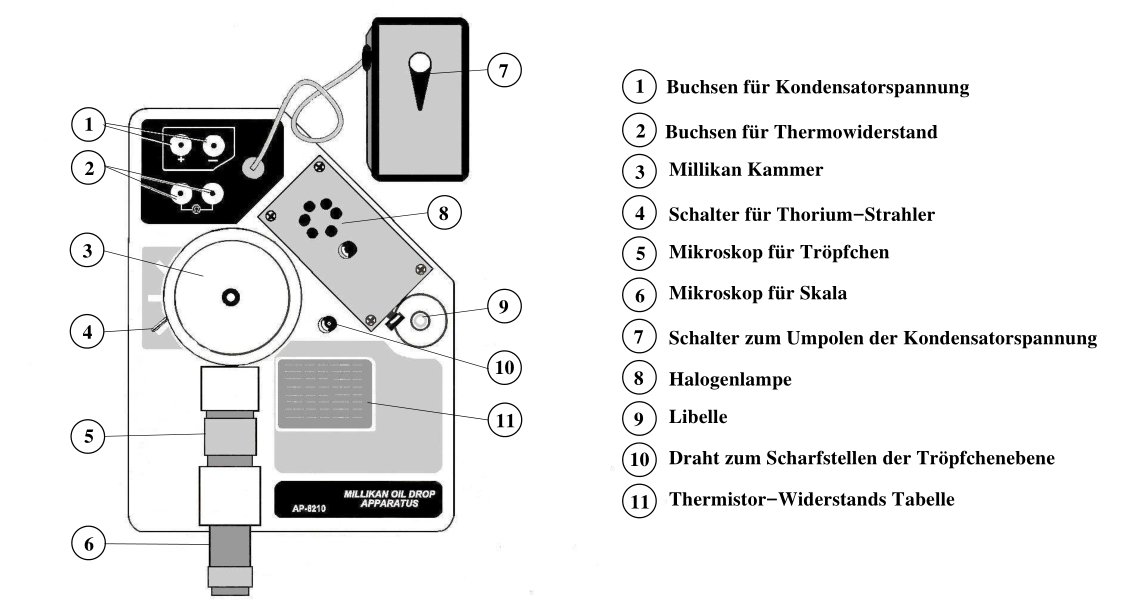
\includegraphics[width = \textwidth]{Pics/Aufbau.png}
  \caption{Experimenteller aufbau \cite{anleitung01}.}
  \label{fig:Aufbau}
\end{figure}

Der experimentelle Aufbau ist in Abbildung \ref{fig:Aufbau} zu sehen. Die Platten des
Kondensators haben einen Abstand von $d$ = $(7.6250 \pm 0.051)\si{mm}$. Durch eine
Öffnung in der oberen Platte kann ein mit dem Zerstäuber erzeugtes Tröpchen in
den Kondensator gelangen. Dort wird es durch eine Halogenlampe angestrahlt, damit
die Bewegung unter einem Mikroskop besser verfolgt werden kann. Die Temperatur in
dem Kondensator kann mit einem Thermowiderstand kontrolliert werden. Um die Ladung
der Tröpchen zu verändern wird ein schwach radioaktives $\alpha$-Präparat($\ce{^{232}Th},
8 \mu Ci$) in die untere Platte eingelassen. Es kan mit dem Hebel (4) abgeschirmt
oder aktiviert werden. Bei der Mitteleinstellung ist das Shutter geöffnet und das
Tröpchen kann in den Kondensator gelangen.

 Die Ausrichtung der Apparatur kann mit der Libelle (9) überprüft werden. Mit einem
 Multimeter kann die angelegte Spannung gemessen werden und mit dem Hebel (7)
 kann die Ausrichtung des elektrischen Feldes bestimmt werden. Da sich die Luft
 aufgrund der Halogenlampe konstant erwärmt, wird der Widerstand des Thermistors
 alle 15 Minuten gemessen, um mit einer Thermistor-Widerstandstabelle die
 Temperatur zu bestimmen.

\subsection{Durchführung}

Als erstes wird mithilfe der Libelle überprüft, ob der experimentelle Aufbau
richtig ausgerichtet ist. Anschließend wird das Mikroskop scharf gestellt, indem
auf das Millimeterpapier fokussiert wird.
%War das wirklich so?

Zuerst werden bei ausgeschaltetem elektrischen Feld Öltröpfchen in den Kondensator
gegeben. Für die Messung der Geschwindigkeit wurde ein Strecke von $\SI{5}{mm}$
betrachtet, bei der die Zurücklegung dieser Strecke optimalerweise in einem Zeitraum
von $ 5 < t < 30 \, s$ geschehen soll. Somit werden nur Teilchen ausgewählt, deren
Geschwindigkeit $v\ua{0}$ zwischen $\SI{0.001}{\meter\per\second}$ und
$\SI{0.00016}{\meter\per\second}$ liegt.

Anschließend wird das elektrische
Feld eingeschaltet, um die Ladung des Tröpchens zu überprüfen. Dafür wird das
Verhalten des Tröpchens bei den verschiedenen Polungen des Kondensators betrachtet.
Sollte das Tröpchen
ungeladen sein, wird bei ausgeschaltetem elektrischen Feld kurzzeitig die Umgebungsluft
mit der radioaktiven Quelle ionisiert, da sich so mehr Elementarladungen auf dem
Tröpchen absetzen.

Sobald ein Tröpfchen mit passender Geschwindigkeit und Ladung gefunden wird, wird
die Spannung des Kondensators so eingestellt, dass das Tröpchen ruht. Diese
Messung wird für insgesamt 30 verschiedene Öltröpfchen wiederholt.
